% SIAM Article Template
\documentclass[review,onefignum,onetabnum]{siamonline171218}

% Information that is shared between the article and the supplement
% (title and author information, macros, packages, etc.) goes into
% ex_shared.tex. If there is no supplement, this file can be included
% directly.
\usepackage{graphicx}
 \usepackage{leftidx}
% SIAM Shared Information Template
% This is information that is shared between the main document and any
% supplement. If no supplement is required, then this information can
% be included directly in the main document.


% Packages and macros go here
\usepackage{lipsum}
\usepackage{amsfonts}
\usepackage{graphicx}
\usepackage{epstopdf}
\usepackage{algorithmic}
\ifpdf
  \DeclareGraphicsExtensions{.eps,.pdf,.png,.jpg}
\else
  \DeclareGraphicsExtensions{.eps}
\fi

% Prevent itemized lists from running into the left margin inside theorems and proofs
\usepackage{enumitem}
\setlist[enumerate]{leftmargin=.5in}
\setlist[itemize]{leftmargin=.5in}

% Add a serial/Oxford comma by default.
\newcommand{\creflastconjunction}{, and~}

% Used for creating new theorem and remark environments
\newsiamremark{remark}{Remark}
\newsiamremark{hypothesis}{Hypothesis}
\crefname{hypothesis}{Hypothesis}{Hypotheses}
\newsiamthm{claim}{Claim}

% Sets running headers as well as PDF title and authors
\headers{Scheduling Multi-source Divisible Loads on an Arbitrary Networks with Granularity Constraints}{Junwei Zhang}

% Title. If the supplement option is on, then "Supplementary Material"
% is automatically inserted before the title.
\title{Scheduling Multi-source Divisible Loads on an Arbitrary Networks with Granularity Constraints\thanks{Submitted to the editors DATE.}}

% Authors: full names plus addresses.
\author{Junwei Zhang\thanks{ 
  (\email{junwei.zhang@stonybrook.edu}).}
}


\usepackage{amsopn}
\DeclareMathOperator{\diag}{diag}


%%%% HELPER CODE FOR DEALING WITH EXTERNAL REFERENCES ON OVERLEAF
% (from an answer by cyberSingularity at http://tex.stackexchange.com/a/69832/226)
%%%
\makeatletter
\newcommand*{\addFileDependency}[1]{% argument=file name and extension
  \typeout{(#1)}% latexmk will find this if $recorder=0 (however, in that case, it will ignore #1 if it is a .aux or .pdf file etc and it exists! if it doesn't exist, it will appear in the list of dependents regardless)
  \@addtofilelist{#1}% if you want it to appear in \listfiles, not really necessary and latexmk doesn't use this
  \IfFileExists{#1}{}{\typeout{No file #1.}}% latexmk will find this message if #1 doesn't exist (yet)
}
\makeatother

\newcommand*{\myexternaldocument}[1]{%
    \externaldocument{#1}%
    \addFileDependency{#1.tex}%
    \addFileDependency{#1.aux}%
}
%%% END HELPER CODE

%%% Local Variables: 
%%% mode:latex
%%% TeX-master: "ex_article"
%%% End: 


% Optional PDF information
\ifpdf
\hypersetup{
  pdftitle={Scheduling Multi-source Divisible Loads on an Arbitrary Networks with Granularity Constraints},
  pdfauthor={Junwei Zhang}
}
\fi

% The next statement enables references to information in the
% supplement. See the xr-hyperref package for details.

%% Use \myexternaldocument on Overleaf
\myexternaldocument{ex_supplement}

% FundRef data to be entered by SIAM
%<funding-group>
%<award-group>
%<funding-source>
%<named-content content-type="funder-name"> 
%</named-content> 
%<named-content content-type="funder-identifier"> 
%</named-content>
%</funding-source>
%<award-id> </award-id>
%</award-group>
%</funding-group>

\begin{document}

\maketitle

% REQUIRED
\begin{abstract}
Many interconnection networks have been proposed and studied in the work to date on divisible load scheduling.

I want to focus on multi-source data injection problem.The practical machines have load injected into their interconnection fabric at multiple points simultaneously.

I want to consider from the following perspectives:

\begin{itemize}
\item The topology of networks: 
\begin{enumerate}
\item linear chain, buses\cite{ko2008signature}, trees\cite{kyong2012greedy}, tori, regular mesh\cite{ying2014signature}, hypercubes\cite{drozdowski1999scheduling},general networks\cite{jia2010scheduling}
\item Kinetic clustering method\cite{ni2016capacitated} which means the user can add/drop some data injection source during the system is running.
\item Constrain of Data injection position. For example, the company need there must be a data injection in one specific location and we can decide the other locations.
\end{enumerate}
\end{itemize}
\begin{itemize}
\item Data property: 
\end{itemize}
\begin{enumerate}
\item Big Chunk Data:  for example the big flat file\cite{ko2008signature}, we try to minimize the total time
\item Streaming Data: for example Surveillance video\cite{eriksson2017distributed} \cite{redondi2015mathematical}, mobile phone camera video stream. Optimize the max flow in the data network in a stable situation.
\item Data has granularity limitation\cite{li2001divisible}
\item Communication Delay.
\item Load Sharing.
\end{enumerate}
\begin{itemize}
\item Node :
\end{itemize}
\begin{enumerate}
\item workstations or sensor node has a limit buffer size\cite{li2001divisible}
\end{enumerate}
\begin{itemize}
\item Method:
\end{itemize}
\begin{enumerate}
\item Superposition\cite{robertazzi2006multi}\cite{krevat2002job}
\item Queue theory. not only consider the M/M/1\cite{ko2002scheduling}, we also can think about the M/M/K  or different data distribution function.  which means some nodes consist of a cluster and share the memory together.
\end{enumerate}
\end{abstract}
% REQUIRED
\begin{keywords}
  divisible load theory, granularity, queuing theory, kinetic clustering, superposition, three-dimensional network 
\end{keywords}

\section{Introduction}

I have implemented four algorithms in the past week, which are queuing theory M/M/1\ref{fig:MM1}, M/M/K \ref{fig:MMK} queue model simulation.
\begin{figure}
\centering
\includegraphics[width=6.5in]{queuelength.eps}
\caption{M M 1 simulation}
\label{fig:MM1}
\end{figure}

\begin{figure}
\centering
\includegraphics[width=6.5in]{Kqueuelength.eps}
\caption{M M K simulation}
\label{fig:MMK}
\end{figure}

I simulate there are total 500 or 900 vehicles comes with \textit{Possion} process, with different  $\lambda$ and $\mu$ . 
In the Fig \ref{fig:MM1}, which indicate that if the coming rate $\lambda$ exceed the service rate $\mu$ the queue length with grows. If the coming rate $\lambda$  is smaller or equals than the service rate $\mu$. The queue length can is small enough.  

In the Fig \ref{fig:MMK}, which simulate there are 900 vehicles come as a \textit{Possion} process and there are $K= 3$ workstations to support the service. We assume each station has the homogeneous processing capacity $\mu$. If the unified ability $\frac{\mu}{K}$is smaller than $\lambda$ , the mean length of the queue is growing. If the unified service capacity is greater than $\lambda$ , the mean length of the queue keeps short.

In addition, I also reproduce the DTL for daisy chain link and single level tree topology.

If the $M = 5$, $w \times Tcp = 1$ and $z \times Tcm = 1$ then the chain DTL $\alpha$ fragment is following

\begin{table}[]
\centering
\caption{$5$ Node Daisy Chain Link fragment ratios under DTL}
\label{my-label}
\begin{tabular}{|l| l| l| l| l| l}
\hline
$\alpha_{0}$ &$\alpha_{1}$  &$\alpha_{2}$  &$\alpha_{3}$  & $\alpha_{4}$  \\
\hline
0.6182 &0.2364  &0.0909  &0.0364  &0.0182  \\
\hline
\end{tabular}
\end{table}

If the $M = 4$, installment $N = 3$ and   $w \times Tcp = 1$ and $z \times Tcm = 1$ then single level tree

$\alpha$ ratio 

\begin{table}[]
\centering
\caption{$4$ Node $3$ installment single level tree fragment ratios under DTL}
\label{my2label}
\begin{tabular}{|l| l| l| l| l| l |l |l |l | l |l |l |l}
\hline
$\alpha_{0}$ &$\alpha_{1}$  &$\alpha_{2}$  &$\alpha_{3}$  & $\alpha_{4}$ & $\alpha_{5}$ &$\alpha_{6}$\\
\hline

0.5000 &0.2407 &0.0174 &0.0013 &0.1249 &0.0090 & 0.0006\\
\hline

$\alpha_{7}$ &$\alpha_{8}$ &$\alpha_{9}$ &$\alpha_{10}$ &$\alpha_{11}$ &$\alpha_{12}$ \\
\hline
0.0648 &0.0047 &0.0003 &0.0336 &0.0024 &0.0002\\
\hline
\end{tabular}
\end{table}


\bibliographystyle{siamplain}
\bibliography{references}

\end{document}
